\section{Моделирование предметной области и разработка функциональных
требований}

{
\renewcommand{\mathbf}[1]{#1}

\subsection{Сенсоры}

Для осуществления задачи навигации необходимо получать знания об окружающей
среде. Это можно осуществить с помощью использоватния различных сенсоры. Каждый
сенсор получает информацию об определённых свойствах окружающей среды и о
свойствах самого робота. Система должна поддерживать использование нескольких
сенсоров для более устойчивого картирования и определения своей позиции.

\subsubsection{LIDAR}

\begin{figure}[h]
\centering
	\fbox{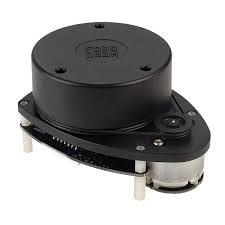
\includegraphics[width=9cm]{2d_lidar}}
\caption{2D LIDAR}
\end{figure}

Сенсор LIDAR выдаёт 2D снимок помещения -- облако точек в двумерной плоскости.
Используя облако точек, и зная позицию в которой снимок облака был совершён,
возможно реконструировать карту окружающего пространства на сетке. Если провести
отметить все клетки через которые прошёл луч лазера за пустые, и отметить последнюю
в которой луч отразился в качестве отмеченной, то получается сетка занятости
(Occupancy Grid).

\subsubsection{IMU}
Сенсор IMU (inertial measurement unit) даёт информацию об угловом и линейном
ускорении, что позволят определять текущее положение в пространстве.
Используя вектор гравитации можно определить направление в которое робот
смотрит, а проинтегрировав угловое ускорение возможно определить текущую
ориентацию.

\begin{figure}[h]
\centering
	\fbox{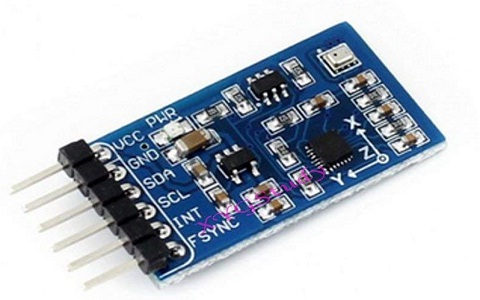
\includegraphics[width=9cm]{IMU}}
\caption{IMU}
\end{figure}

\subsubsection{GPS}
Сенсор GPS выдаёт глобальную позицию в мировых координатах. Типичная точность
современных GPS-приёмников составляет 6-8 метров при хорошей видимости
спутников, что недостаточно для автономной навигации, но GPS всё ещё можно
использовать в качестве дополнительно источника данных для фильтрации.
Отличительной особенностью GPS является то, что он измеряет положение в
абсолютных величинах и не подвержен постепенному накоплению ошибки.

\subsection{Шасси}
Для задачи навигации неважно какое шасси используется, главное чтобы была
возможность достигать указанной угловой и линейной скорости. Программное
средство должно отправлять данные о желаемой угловой и линейной скорости, а
реализация движения зависит от того на какой конкретно мобильной системе
программное средство будет использоваться

\subsection{Общие сведения и требования к работе программного средства}

Для визуализации конечных требований к системе воспользуемся UML диаграммой
вариантов использования. (Рис. \ref{pic:usecase})

\begin{figure}[h]
\centering
	\fbox{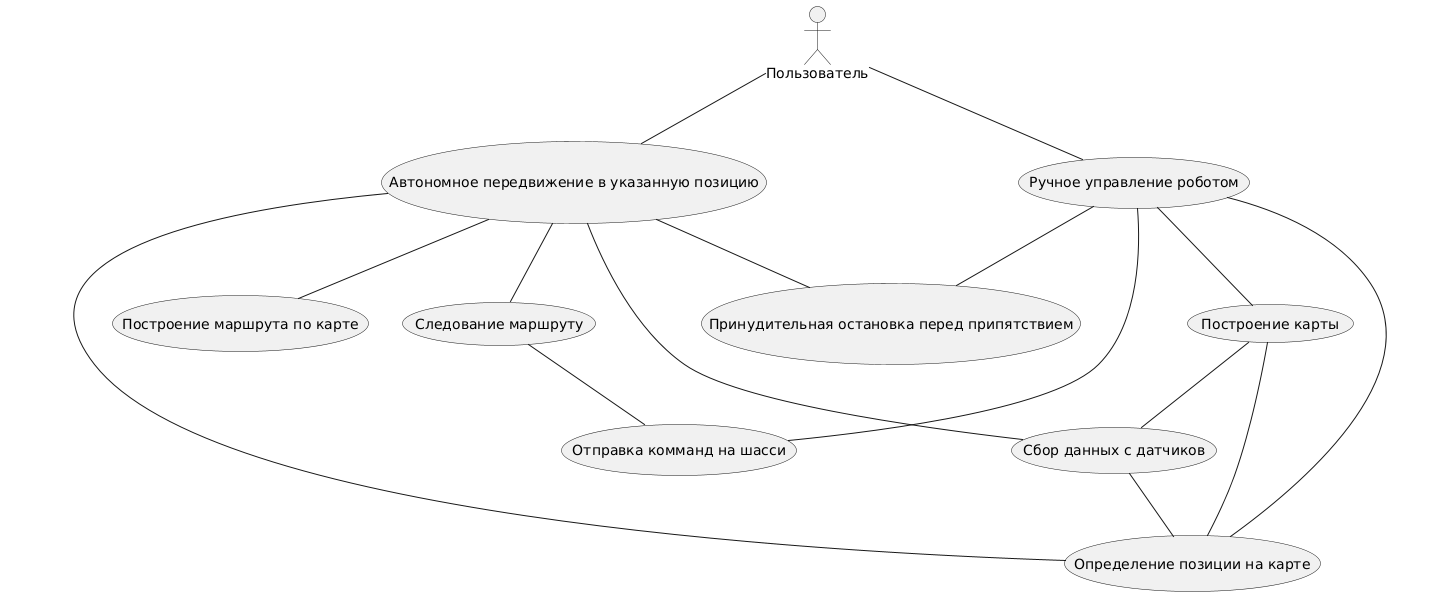
\includegraphics[width=15cm]{UML}}
\caption{Usecase диаграмма программного средства}
	\label{pic:usecase}
\end{figure}

Сделаем вывод, что программное средство должно:

\begin{itemize}
	\item принимать и обрабатывать данные с сенсоров;
	\item определять текущее местоположение;
	\item строить карту окружающего пространства;
	\item строить маршрут из текущей позиции в указанную пользователем;
	\item на основе построенного маршрута отправлять команды на шасси, учитывая
		окружающие препятствия;
	\item избегать столкновений.
\end{itemize}

%
% % \subsection{Описание функциональности программного средства}
% %
% % \todo{USECASE диаграмма}
% % \subsection{Спецификация функциональных требований}
%
% - Моделируем навигацию
% - Occupancy grid
% - Надо переместится в указанную точку на карте
% - Способ указывания точки на карте
%
% % \todo{ Если цель переместится в указанную точку, для этого надо построить
% % маршрут, чтобы построить маршрут нужна карта, чтобы построить карту используем
% % позицию и показания с сенсоров и метод SLAM }

\subsection{Разработка функциональных требований к проектируемому программному
средству}
% WATER
	Для успешной реализации системы мобильной навигации необходимо четко
	определить и описать функциональные требования, которые будут обеспечивать
	эффективность и точность работы системы. Эти требования являются основой для
	проектирования и разработки как аппаратной, так и программной части системы.
	В данном разделе рассматриваются ключевые аспекты, которые должны быть
	учтены при разработке функциональных требований для мобильной навигации,
	включая работу с картами, выполнение маршрутов и интеграцию различных
	сенсоров.

Система должна:
\begin{itemize}
	\item получать данные с сенсоров IMU, GPS, LIDAR;
	\item обрабатывать полученные данные и определять текущую позицию;
	\item строить карту окружающей среды;
	\item строить и выполнять маршут перемещаясь в указанную позицию;
	\item сохранять и загружать построенную карту между запусками;
\end{itemize}

\subsection{Разработка технических требований к программному средству}

Разрабатываемое программное решение должно обеспечивать корректное
функционирование при развёртывании на компьютерном модуле BananaPi CM4, или
на модуле со следующими техническими характеристиками:

\begin{itemize}
	\item оперативная память 4 Гбайт или более;
	\item amlogic A311D шести ядерный процессов с четырьмя Arm Cortex-A73
		ядрами, двумя Arm Cortex-A53 ядрами, или более быстродействующий
		процессор;
	\item доступный объём дискового пространства 5 Гбайт. %20mb на самом деле
\end{itemize}
